\documentclass[11pt, a4paper, spanish, openright, twoside]{book}
\usepackage[spanish, activeacute]{babel}
\usepackage[utf8]{inputenc}
%\usepackage[top=2.5cm, bottom=2.5cm, outer=1.75cm, inner=1.75cm, heightrounded, marginparwidth=2.5cm, marginparsep=0.3cm]{geometry}	%márgenes empequeñecidos
\usepackage[top=2.95cm, bottom=2.25cm, outer=2.75cm, inner=2.75cm, heightrounded, marginparwidth=2.5cm, marginparsep=0.3cm]{geometry}	%márgenes originalmente
\usepackage{dpg}
\usepackage{fli}

\usepackage{pgf}
\usepackage{tikz}

\usepgflibrary{shapes.geometric} % LATEX and plain TEX and pure pgf
\usetikzlibrary{arrows,automata,positioning}
\tikzstyle{accepting by double}= [double distance=1.6pt,double,outer sep=.5\pgflinewidth+.8pt] % esto es algo estético.
\renewcommand\shorthandsspanish{}  % para compatibilizar spanish con tikz

%%%%%%		Figuras		%%%%%%%%%%%%%%%%%%%
\usepackage[vflt]{floatflt}		%Entorno float-figure

%%%%%%		Page style		%%%%%%%%%%%%%%%%%%%
\renewcommand{\thepage}{\arabic{page}}% Arabic page numbers\fancyhead{}
\pagestyle{fancy}
\fancyfoot{}
\fancyhead[LO,RE]{Práctica 4}	%encabezado de pares: nombre de la sección
\fancyhead[RO,LE]{Búsqueda de rutas en un mapa utilizando la librería AIMA}
\fancyfoot[LE,RO]{\thepage}	%abajo a izqda en pares, derecha en impares: numero de pagina
%\fancyhead[LE]{\nouppercase{\leftmark}} %cuadro izquierdo de pagina par: parte y contador
\fancyfoot[CE]{Inteligencia Artificial} 
\fancyfoot[CO]{Doble Grado Informática-Matemáticas - Universidad Complutense}
\renewcommand{\footrulewidth}{0.4pt}
\renewcommand{\headrulewidth}{0.4pt}		% linea por debajo del encabezado
\renewcommand{\sectionmark}[1]{\markright{\textbf{\thesection. #1}}}	%negrita
\renewcommand{\labelitemi}{$\circ$} %Primer itemize con circunferencia vacia
\renewcommand{\labelitemii}{$\cdot$} %Segundo itemize con punto pequeño \cdot
\renewcommand*{\thesection}{\arabic{section}}	% Hace que no apareca el indice de capitulos y que comience en section

%%%%%%		Others		%%%%%%%%%%%%%%%%%%%
\setlength{\leftmarginii}{0em} %Segundo itemize sin sangria
\setlength{\leftmarginiii}{1em} %Tercer itemize casi sin sangria
\renewcommand{\labelitemiii}{ }
\pagenumbering{roman}
\addto{\captionsspanish}{\renewcommand*{\contentsname}{Índice}} %Cambia "Indice general" por "Indice"



\begin{document} 
\title{\Huge{\textsc{Inteligencia Artificial}} \\
	\vspace{0.7cm}
	 \textsc{\Large{Práctica 4}} \\
	\vspace{1.5cm}
	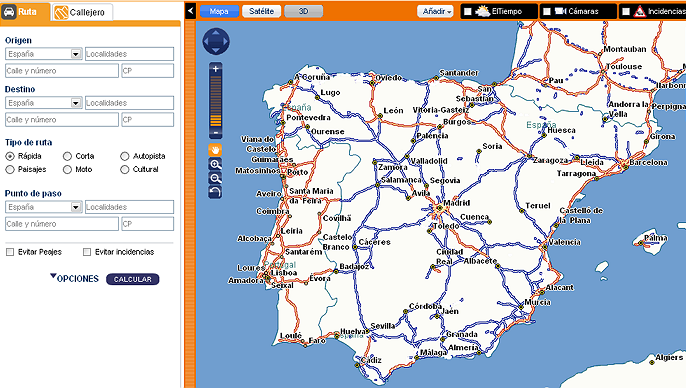
\includegraphics[scale=0.45]{mapaCarreteras}}
\author{\textsc{Grupo 3:}\\
	Enrique Ballesteros Horcajo\\
	Ignacio Iker Prado Rujas}
\date{\Today}
\maketitle

\newpage
\mbox{}
\thispagestyle{empty}						% Hoja en blanco, sin numeros ni nada
\newpage


\tableofcontents 							%INDICE hipervinculado

\newpage
\mbox{}
\thispagestyle{empty}						% Hoja en blanco, sin numeros ni nada
\newpage

\pagenumbering{arabic}						% Pone el contador de paginas a 1 y ahora en numeros normales

\vspace{3cm}


\newpage



\begin{section}{Introducción: Mapa de carreteras}

	\textbf{Problema:} 
	
	\textit{El objetivo de esta práctica es aplicar aima.core y aima.gui a la búsqueda de rutas entre capitales de provincias de las comunidades de Castilla-León, Castilla-La Mancha y Madrid. }
	
	\textit{Para representar el mapa utiliza un grafo no dirigido con suficiente número de nodos y aristas para que existan rutas alternativas (no es necesario representar todas las ciudades ni todas las carreteras). }
	
	\textit{Para construir el mapa de España simplificado empieza eligiendo una serie de capitales de provincia de las regiones indicadas (incluyendo Madrid) y obteniendo sus coordenadas UTM\footnote{Sistema de coordenadas Universal Transversal de Mercator} en aplicaciones específicas como \url{http://www.maps.pixelis.es/}. A partir de estas coordenadas en kilómetros, calcula las coordenadas relativas a la ciudad de Madrid, que se utilizará como punto central de la representación gráfica, restando a las coordenadas de cada ciudad las coordenadas de Madrid. Además extrae de \url{https://maps.google.es/} las longitudes de las rutas directas entre las capitales cercanas entre sí. Una ruta directa entre dos capitales es la que no pasa por ninguna otra capital de provincia. Como máximo se seleccionará una ruta directa entre cada dos capitales, representándola como una arista bidireccional en el grafo.}


\end{section}

	\begin{section}{Ciudades y carreteras de España. Coordenadas UTM}
		A partir de las coordenadas UTM de cada ciudad, obtenemos sus coordenadas relativas respecto a Madrid.
		\begin{itemize}
		\item Madrid	(440, 4475)		\textrightarrow	(0, 0)

		\item Toledo	(410, 4415)		\textrightarrow	(-30, -60)
		\item Guadalajara	(485, 4500)	\textrightarrow	(45, 25)
		\item Cuenca	(570,  4435)		\textrightarrow	(130, -40)
		\item Albacete	(600, 4315)	\textrightarrow	(160, -160)
		\item Ciudad Real 	(420, 4315)	\textrightarrow	(-20, -160)

		\item Soria	(540, 4625)		\textrightarrow	(100, 150)
		\item Palencia	(370, 4650)  	\textrightarrow	(-70, 175)
		\item Segovia	(405, 4535)	\textrightarrow	(-35, 60)
		\item Valladolid	(355, 4610)	\textrightarrow	(-85, 135)
		\item Salamanca	(275, 4540)	\textrightarrow	(-165, 65)
		\item Burgos	(440, 4690)		\textrightarrow	(0, 215)
		\item Zamora	(270, 4600)		\textrightarrow	(-170, 125)
		\item Ávila	(355, 4500)		\textrightarrow	(-85, 25)
		\item Tomelloso	(500, 4330)  	\textrightarrow	(60, -145)
		
		\item Cáceres(725, 4370)		\textrightarrow	(285, -105)	
		\item Barcelona(430, 4580)	\textrightarrow	(-10, 105)

		\end{itemize}

		Y desde google maps obtenemos la longitud de las carreteras que las unen. Vamos a poner pocas carreteras para que el análisis sea más sencillo:

			\begin{itemize}
				\item MADRID-AVILA, 108 km.
				\item MADRID-SEGOVIA, 93 km.
				\item MADRID-GUADALAJARA, 60 km.
				\item MADRID-TOLEDO, 72 km.
				\item MADRID-CUENCA, 170 km.
				\item AVILA-SALAMANCA, 110 km.
				\item SALAMANCA-ZAMORA, 65 km.
				\item ZAMORA-VALLADOLID, 100 km.
				\item VALLADOLID-SEGOVIA, 120 km.
				\item VALLADOLID-PALENCIA, 50 km.
				\item PALENCIA-BURGOS, 90 km.
				\item SORIA-BURGOS, 140 km.
				\item GUADALAJARA-SORIA, 170 km.
				\item CUENCA-ALBACETE, 160 km.
				\item TOLEDO-CIUDAD REAL, 120 km.
				\item CIUDAD REAL-TOMELLOSO, 90 km.
				\item ALBACETE-TOMELLOSO, 130 km.

	
			\end{itemize}
	\end{section}
	\begin{section}{ ¿Qué pasaría si añadiéramos al mapa la ciudad de Cáceres. ¿Sería correcta su situación? ¿Por qué?}
		Al colocar Cáceres con sus coordenadas relativas UTM respecto a Madrid, observamos que su coordenada correspondiente 
		a la $x$ es positiva: esto quiere decir que en nuestro mapa Cáceres estará a la derecha de Madrid. Por tanto, la situación de Cáceres 
		en el mapa no sería correcta.

		Lo primero decir que no solo pasa con Cáceres,  con más ciudades (como Barcelona) también obtenemos unas coordenadas relativas incorrectas. Para explicar por qué ocurre esto basta echar un vistazo a la siguiente imagen que nos muestra los cuadrantes UTM en
		el mapa.

	\begin{center}
		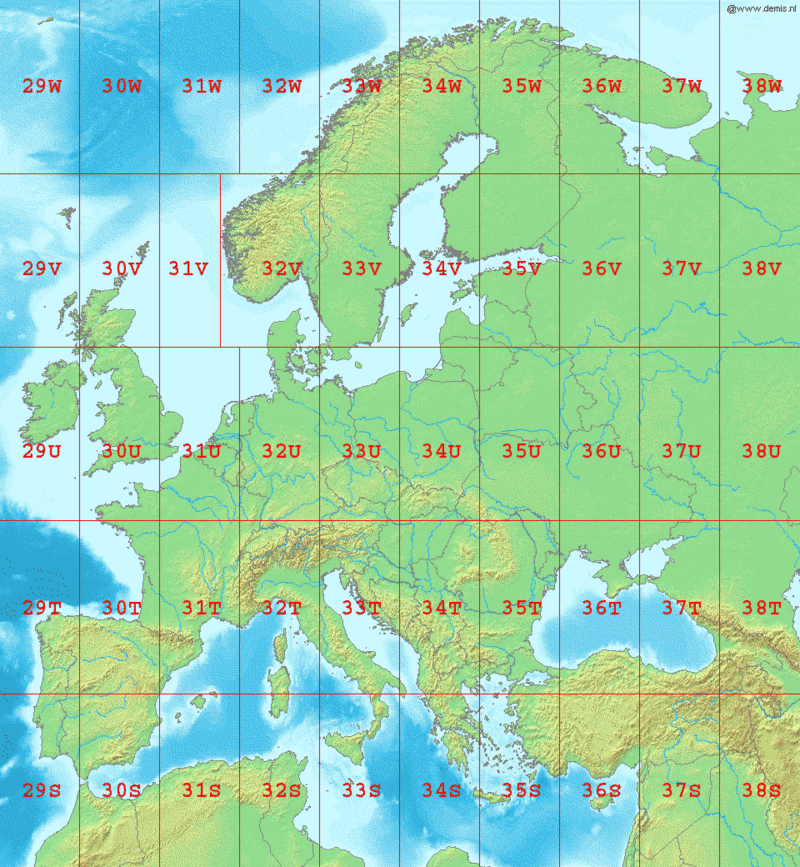
\includegraphics[scale=0.45]{mapaUTM}
	\end{center}

		Como puede verse, Barcelona y Cáceres están en cuadrantes distintos a Madrid.
		Esto se debe a que pertenecen a distintos husos. Barcelona está en el huso 31, Madrid en el 30 y Cáceres en el 29. Al cambiar de uso, 
		las coordenadas UTM pertenecientes a la 'x' cambian. Así, Castellón de la Plana tiene coordenadas (752 ,  4431 ,  30 ) y su puerto (245  ,  4430, 31) 
		cuando distan 8 kilómetros el uno del otro.

	\end{section}

	\begin{section}{¿Cómo se podría aplicar el código desarrollado en esta práctica a un mapa de calles de una ciudad? Describe qué información tendrías que representar y cómo lo harías.}
		El concepto base es el mismo, por lo que podría aplicarse el mismo código. Esto siendo un mapa simplificado también. Igual que hemos supuesto en nuestro mapa que las carreteras que unen ciudades son
 		bidireccionales y tienen la misma longitud de ida y de vuelta, necesitaríamos que las calles de la ciudad fuesen todas bidireccionales. Este es el mayor problema que presenta el aplicar nuestro código. A diferencia 
		de carreteras que unen ciudades, que siempre existen en ambas direcciones (si bien no tienen la misma longitud), en las calles suele darse el caso de que son unidireccionales: solo pueden recorrerse en un sentido.
		 
		Si salvamos este punto, podríamos aplicar nuestro código de la siguiente forma: cada ciudad pasa a ser una plaza o un cruce de calles. Cada carretera que antes unía ciudades  pasa a ser una calle que une dos 
		plazas o dos cruces. Ahora tenemos el problema de que la misma calle une plazas consecutivas, pero esto solo afecta si damos nombres a las calles y las carreteras. En nuestra práctica solo identificamos una carretera por 
		la longitud que tiene y las ciudades que une. De esta manera, una vez identificados los cruces de nuestra ciudad basta unirlo por las calles correspondientes y no tendremos ningún problema.
		
		Otro tema importante en las ciudades son los semáforos, pero a partir de  la modificación que nos permite incluir el tráfico podemos añadir otra que nos incorpore el tiempo medio en cruzar una calle teniendo en cuenta 
		los semáforos. 

		Por tanto, representando la dirección del tráfico de las calles (parte nueva en nuestro código), representando los cruces de calles y las calles que los unen, tendríamos un mapa de calles de una ciudad. 		


	\end{section}
	
\begin{thebibliography}{9}

\bibitem{aima}
	Russell, S.; Norvig, P, \\
	\emph{Artificial Intelligence, a modern aproach}.\\
	New Jersey: Pearson, 2010.
	
\bibitem{clase}
	Apuntes y transparencias de Inteligencia Artificial, \\
	Doble Grado Matemáticas - Ing. Informática, U.C.M., 2014-2015.

\end{thebibliography}


\end{document}

